\documentclass[a4paper]{article} 
\addtolength{\hoffset}{-2.25cm}
\addtolength{\textwidth}{4.5cm}
\addtolength{\voffset}{-3.25cm}
\addtolength{\textheight}{5cm}
\setlength{\parskip}{0pt}
\setlength{\parindent}{0in}

%----------------------------------------------------------------------------------------
%	PACKAGES AND OTHER DOCUMENT CONFIGURATIONS
%----------------------------------------------------------------------------------------

\usepackage{blindtext} % Package to generate dummy text
\usepackage{charter} % Use the Charter font
\usepackage[utf8]{inputenc} % Use UTF-8 encoding
\usepackage{microtype} % Slightly tweak font spacing for aesthetics
\usepackage[english, ngerman]{babel} % Language hyphenation and typographical rules
\usepackage{amsthm, amsmath, amssymb} % Mathematical typesetting
\usepackage{float} % Improved interface for floating objects
\usepackage[final, colorlinks = true, 
            linkcolor = black, 
            citecolor = black]{hyperref} % For hyperlinks in the PDF
\usepackage{graphicx, multicol} % Enhanced support for graphics
\usepackage{xcolor} % Driver-independent color extensions
\usepackage{marvosym, wasysym} % More symbols
\usepackage{rotating} % Rotation tools
\usepackage{censor} % Facilities for controlling restricted text
\usepackage{listings, style/lstlisting} % Environment for non-formatted code, !uses style file!
\usepackage{pseudocode} % Environment for specifying algorithms in a natural way
\usepackage{style/avm} % Environment for f-structures, !uses style file!
\usepackage{booktabs} % Enhances quality of tables
\usepackage{tikz-qtree} % Easy tree drawing tool
\tikzset{every tree node/.style={align=center,anchor=north},
         level distance=2cm} % Configuration for q-trees
\usepackage{style/btree} % Configuration for b-trees and b+-trees, !uses style file!
\usepackage[backend=biber,style=numeric,
            sorting=nyt]{biblatex} % Complete reimplementation of bibliographic facilities
\addbibresource{ecl.bib}
\usepackage{csquotes} % Context sensitive quotation facilities
\usepackage[yyyymmdd]{datetime} % Uses YEAR-MONTH-DAY format for dates
\renewcommand{\dateseparator}{-} % Sets dateseparator to '-'
\usepackage{fancyhdr} % Headers and footers
\pagestyle{fancy} % All pages have headers and footers
\fancyhead{}\renewcommand{\headrulewidth}{0pt} % Blank out the default header
\fancyfoot[L]{} % Custom footer text
\fancyfoot[C]{} % Custom footer text
\fancyfoot[R]{\thepage} % Custom footer text
\newcommand{\note}[1]{\marginpar{\scriptsize \textcolor{red}{#1}}} % Enables comments in red on margin

%----------------------------------------------------------------------------------------

\begin{document}

%-------------------------------
%	TITLE SECTION
%-------------------------------

\fancyhead[C]{}
\hrule \medskip % Upper rule
\begin{minipage}{0.295\textwidth} 
\raggedright
\footnotesize
Jaime Andres Torres Bermejo \hfill\\   
202014866\hfill\\
andrestbermejoj@gmail.com
\end{minipage}
\begin{minipage}{0.4\textwidth} 
\centering 
\large 
Proyecto 1\\ 
\normalsize 
Diseño y Análisis de Algoritmos\\ 
\end{minipage}
\begin{minipage}{0.295\textwidth} 
\raggedleft
\today\hfill\\
\end{minipage}
\medskip\hrule 
\bigskip

%-------------------------------
%	CONTENIDO
%-------------------------------
\section{Enunciado del Proyecto}


\paragraph{Problema:}

%------------------------------------------------
\section{Especificaciones del proyecto}

\subsection{}

\subsection{Entorno de Desarrollo y entorno de prueba.}

La solución propuesta fue probada en el siguiente entorno de Desarrollo, debería funcionar en
computadores que compartan las dependencias principales, Java (del cual se probó en Java 17 y en Java 1.8) o un sistema operativo basado
en Unix, así no comparta necesariamente el hardware. No se proporciona un entorno de virtualización
por lo que recomiendo intentar correrlo en un entorno relativamente similar.

\begin{itemize}
    \item \textbf{Sistema Operativo: } Ubuntu/Kubuntu 22.10 x86\_64, Minimal Install. También probado con Manjaro Linux 22.0 x86\_64 y Fedora
    Linux 38 Workstation Beta x86\_64, por lo tanto se sabe que el programa en teoría podría correr en distribuciones basadas en Debian,
    Red Hat Linux o Arch Linux, no tengo un computador con Mac OS X o BSD para probar con otros sistemas Unix
    \item \textbf{Kernel: }Linux 5.19.0-38-generic
    \item \textbf{Lenguaje de Programación: }Python 3.10.7 x86\_64, Compilado desde apt como un .deb, incluye python3-pip,
    También probado con la versión de Arch y DNF (el manejador de paquetes de Fedora/RHEL)
    \item \textbf{Librerías Utilizadas}
    \begin{itemize}
        \item os
        \item functools
    \end{itemize}
    \item \textbf{Procesador: }AMD Ryzen 5 3550H with Radeon Vega Mobile Gfx (8) @ 2.100GHz 
    \item \textbf{IDE: } Visual Studio Code 1.76.2, instalado desde un paquete snapd. Incluye extensiones
    de Git y Python. En Manjaro fue instalado desde el AUR con el paquete visual-studio-code-bin
\end{itemize}

\subsection{Estructura del Input y Output}
A primera vista, este pareciese ser un problema bastante extraño, si fuesemos a tomarlo por la lógica
del propio problema sin necesariamente cuestionarla. Sin embargo, esta estructura puede verse de forma mucho
más clara al ver la forma como un input esta estructurado, y a partir de esto, comprobar la
utilidad de cada parte del input. Entonces, tomemos como ejemplo el segundo test proveido por el
enunciado:
\begin{verbatim}
    3 
    3 5 8 7 3 4 11
    2 3 4 7 9 
    2 4 5 7 8 4
\end{verbatim}
Y de este input, tendríamos este output:
\begin{verbatim}
    True [(8,3),(7,4),(11)]
    False
    True [(5,7)(8,4)]
\end{verbatim}
Para entender el porque de este output, vamos a tomar el primer input de este
set de inputs:
\begin{verbatim}
    3 5 8 7 3 4 11
    True [(8,3),(7,4),(11)]
\end{verbatim}
La primera cosa a notar es que este input no tiene toda la lista que se pasa por
parámetro. Los dos primeros numeros de la lista se obvian porque \textbf{No representan
familias, sino otras variables que nos serán relevantes.} Especificamente, el primer valor
representa las \textit{k} instancias de CAD, que serán listas, y el segundo valor representa
las \textit{i} familias que existen dentro del sistema, cuyo numero de miembros es
el int que representan. Por lo tanto, el input se vería, una vez formateado, así:
\begin{align*}
    Input = \begin{cases}
        i = 5 \\
        k = 3 \\
        nums = [8, 7, 3, 4, 11]
    \end{cases}
\end{align*}
notese que \textit{i} coincide con la longitud de \textit{nums}, y \textit{k} coincide
con la cantidad de listas generadas en el output. Esto no es una coincidencia, y será muy
importante cuando hablemos del diseño de la solución, pero por ahora, limitemonos a pensar
en que esto cambia la forma en la que pensamos del concepto de CADS y familias, a listas Y
enteros, entonces cuando pensamos el problema, no nos centramos en el enunciado, sino en su 
abstracción, \textbf{si encontramos las \textit{k} tuplas de los valores de nums con suma igual,
resolveremos el problema.}

Para corroborar esto, vamos a tomar la lista del output y vamos a ordenarla
\begin{align*}
    output[1] &= [(8,3), (7,4), (11)] \\
    <suma (Aritmetica)> \\
    output[1] &= [\underset{11}{\underbrace{[3 + 8]}},
    \underset{11}{\underbrace{[7 + 4]}},
    \underset{11}{\underbrace{[11]}}]
\end{align*} 

Como es posible tomar la lista \textit{nums} y ponerla en \textit{k} tuplas de
sumas exactamente iguales, entonces el resultado es True, si no fuese posible, simplemente
se retornaría False, la estructura dinámica de Python y sus retornos nos permitirá hacer
de forma bastante sencilla la solución, pero nos estamos adelantando.

\subsection{Lectura de datos}
Según se nos fue informado por los monitores, la lectura se hará a partir de la lectura
de archivos de texto y, por lo tanto, la estructura del archivo de Python esta pensada para
poder leer varios archivos de texto secuencialmente. Para esto hemos importado la librería 'os'
de las librerías base de Python, con esta y el 
%------------------------------------------------
\section{Diseño de la Solución}
\subsection{Conceptos Teóricos Importantes}
\subsubsection{Programación Dinámica}

\subsubsection{Operaciones in-place}
En Python, se pueden definir operaciones In-place con el operador 
\begin{verbatim}
    '|=' en lugar de '='
\end{verbatim}
el uso de esta notación nos permite ahorrar
memoria a la hora de escribir código, al usar la misma dirección de memoria para
almacenar el resultado, sin necesidad de hacer una nueva dirección en memoria. aunque
lenguajes de menor nivel, como C++ o Rust (este último al que estoy contribuyendo) nos
permiten hacer algunas operaciones de manera implicitamente in-place, la naturaleza 
interpretada de Python hace que el manejo de estos sistemas deba escribirse explicitamente
para forzar al compilador a consistentemente procesar la acción como in-place.


\subsubsection{Memorización}
La Memorización se define cómo: 'a'[2]

\subsection{Conceptos Prácticos Importantes}
\subsubsection{Tipado dinámico}
El lenguaje de Programación utilizado para resolver este algoritmo fue Python,
el cuál tiene la capacidad de mantener una estructura de tipado dinámica, esta
implica que podemos declarar una variable de un tipo y esta podrá ser interpretada
como de otro tipo a la hora de compilar el código, otros lenguajes de Programación
con esta caráccteristica son Ruby y Javascript

\subsubsection{Return vacío}
Python nos permite hacer un return nulo, esto puede ser utilizado para imprimir el
resultado de una operacion sin necesidad de preocuparnos por el retorno de este en un
entorno recursivo.

\subsection{Problemas similares}
\subsubsection{Leetcode 416. Partition Equal Subset Sum}
El problema de este proyecto esta pensado como, en realidad, una generalización
del problema 416 de Leetcode, Partition Equal Subset Sum[3], el cual se lee de la siguiente manera:

\begin{verbatim}
    Given an integer array nums, return true if you can partition the array
    into two subsets such that the sum of the elements in both subsets is 
    equal or false otherwise.

    //Example 1
    Input: nums = [1,5,11,5]
    Output: true
    Explanation: The array can be partitioned as [1, 5, 5] and [11].

    //Example 2
    Input: nums = [1,2,3,5]
    Output: false
    Explanation: The array cannot be partitioned into equal sum subsets.
\end{verbatim} 

El problema resuelto en este Proyecto puede considerarse como una generalización en
K subarreglos de este problema, y por eso mismo nos concierne la estructura de esta 
solución para poder entender la forma como se pudo generalizar de 2 subarreglos a \textit{k}
subarreglos.

\paragraph{Estrategia de solución}
Al leer las soluciones propuestas del problema, nos vamos a dar cuenta de dos 
técnicas ampliamente usadas: Top-Down y Memorización. Las definiciones de estos 
términos estan dadas en la sección 3.1 de este documento, pero fuera de lo que son,
Estas dos opciones son generalmente favorecidas sobre una solución de fuerza bruta debido a que:

\begin{itemize}
    \item Puede utilizar soluciones anteriores sin calcularlas otra vez
    \item Evalúa todos los casos posibles sin redundancia
    \item Mantiene un registro que podemos utilizar sin mucho problema
\end{itemize}

En otras palabras, este es un problema que requiere mantener un registro de todos los problemas
solucionados por el algoritmo implementado. Para ver como esto se puede pensar, voy a 
poner 2 de las soluciones propuestas por el post de solución mejor puntuado en Leetcode:[4]

\paragraph{Primera Solución: DP/Memorización Pura / Tabulación}

\begin{verbatim}
class Solution:
    def canPartition(self, nums):
        total_sum = sum(nums)
        if total_sum & 1: return False
        half_sum = total_sum // 2
        dp = [True] + [False]*half_sum
        for num in nums:
            for j in range(half_sum, num-1, -1):
                dp[j] |= dp[j-num]
        return dp[half_sum]
\end{verbatim}

Esta solución nos muestra la forma mas concreta de implementar DP, 
a partir del uso de una estructura de datos que nos permite 

\textbf{Resultados:}

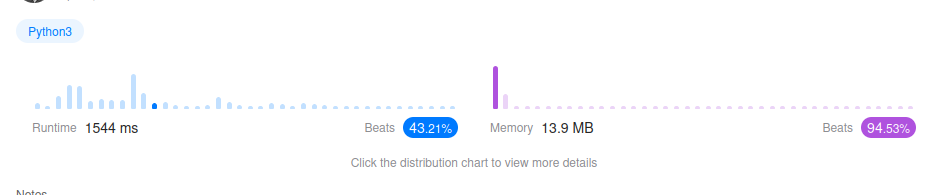
\includegraphics[scale=0.7]{R1.png}

\paragraph{Segunda Solución: DP/Bitmask}
\begin{verbatim}
class Solution:
    def canPartition(self, nums):
        total_sum = sum(nums)
        if total_sum & 1: return False
        half_sum, dp = total_sum // 2, 1
        for num in nums:
            dp |= dp << num
        return dp & 1 << half_sum
\end{verbatim}

Esta segunda solución nos muestra una optimización de tiempo de ejecución importante
de la solución con respecto a tiempo de ejecución. esta optimización se basa en el uso
de una estructura de bits que nos permite ahorrar espacio y hacer operaciones computacionalmente
mas simples, aunque tal vez mas abstractas para el cerebro humano. Entonces tomemos
la idea de la tabla de la solución anterior. Tengamos entonces en cuenta este caso,
sacado de la fuente:

\textbf{Resultados:}

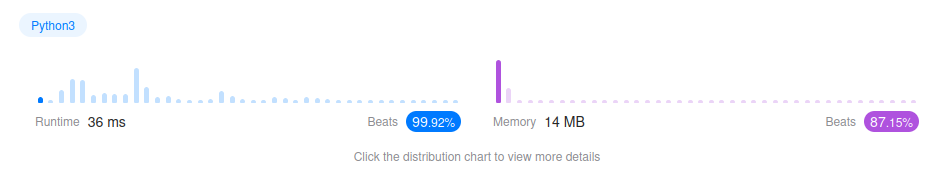
\includegraphics[scale=0.7]{R2.png}

\paragraph{Diferencias con el problema acá planteado}
Dado que estamos generalizando el problema a la hora de hablar de i familias en k CADs, los
casos base propuestos en este problema no pueden ser aplicados, ya que de por si mismos no 
nos garantizan la correctitud del problema. Por ejemplo, pensemos en el caso base:
\begin{verbatim}
    //si la suma total de nums es impar, retorna false  de forma automática
    if(total_sum%2): return False 
\end{verbatim}
Este caso no nos va a servir dentro de la lógica de nuestra solución porque el 
valor de k puede ser mayor a 2, y por esto, pueden forzarse situaciones en las que la suma total
sea impar y el resultado sea 'True', con el fin de entender esto, considerese este
contraejemplo a partir del test 1:

    $$Lemma 1: (totalSum\%2) = False $$
    $$Lemma 2: [8, 7, 3, 4, 11] \rightarrow True \land [(8,3),(7,4),(11)] $$
    $$< Lemma 1, \ True \land q = True, \ Lemma 2, \ 0 = Boolean \ False >$$ 
    $$  True \rightarrow totalSum([8, 7, 3, 4, 11])\%2 = 0$$
    $$<totalSum([8, 7, 3, 4, 11])>$$ 
    $$True \rightarrow 33\%2 = 0$$
    $$<33\%2 = 1 , \ 1 = Boolean \ True, \ Lemma 2>$$ 
    $$True \rightarrow False$$
    $$<True \ can't \ imply \ False>$$
    $$False$$

Por lo tanto, no podemos esperar que todos los casos sean divisibles por 2, y aunque
una solución de este Leetcode nos podría resolver una cantidad limitada de casos, no podemos
subsistir de su lógica completamente con el fin de resolver este problema, pues causará 
falsos negativos en casos donde la suma sea impar.

\subsection{La Solución}
\subsubsection{Mantras de diseño}
\begin{itemize}
    \item \textbf{Hay una suma superior: }La máxima suma que puede ser válida corresponde
    a la suma de todo el array, a partir de esto podemos hacer parte de la tabulación.
    Esto se debe a que por el enunciado, sabemos que los números serán enteros positivos.
    \item \textbf{Debemos poder mantener registro de las sumas: } No solo debe verse el 
    registro de si una suma es posible, sino de las tuplas que lo hacen posible.
\end{itemize}



%------------------------------------------------
\section{Análisis de la Solución}

\subsection{Complejidad}

\subsection{Limitantes}
    \begin{itemize}
        \item el archivo solo puede recibir inputs de archivos de texto, un input no
        puede ser ingresado directamente desde el usuario a partir de la consola
        \item es posible que el programa muera intentando analizar subcarpetas de su carpeta
        de ingreso, por lo que se recomienda mantener los archivos de prueba en el entorno
        raíz de la carpeta 'tests'.
        \item Con el fin de que se pueda abrir en diferentes computadores usamos una ruta relativa
        a la hora de escribir el entorno de ficheros de donde tomará las pruebas, si se usa este 
        para calificar, es necesario abrir en el entorno desde la primera carpeta del proyecto en
        caso de usar un IDE, se puede modificar la ruta de lectura, caso en el cuál debería poderse. 
    \end{itemize}
\subsection{Consideraciones}
\begin{itemize}
    \item La capacidad de tipado dinámico de Python es directamente responsable de
    la capacidad de este algoritmo en algunos casos, gran parte de las funciones
    de carácter lambda deberían reescribirse en caso de que se fuese a reescribir la solución
    en un sistema de tipado estático.
    \item se omite la primera linea del archivo que leemos porque se asume tiene la
    cantidad de casos de prueba necesarios para el archivo, esta información nos
    sería relevante en lenguajes como C, donde se debe configurar manualmente el manejo
    de ciclos en situaciones como esta.
    \item A día de hoy, este es un trabajo en grupo que realicé solo, por favor ten eso
    en cuenta, profe.
\end{itemize}
%------------------------------------------------
\section{Referencias.}
\begin{itemize}
    \item [1]: \textit{Enunciado del proyecto, ISIS 1105 Diseño y Análisis de Algoritmos
    Semestre 2023-10. Proyecto – PARTE 1} Uniandes, 2023.
    \item [2]: \textit{The Algorithm Design Manual, Springer, Second Edition}, Steven S. Skiena, 2008.
    \item [3]: \textit{416. Partition Equal Subset Sum}, Leetcode, recuperado de 
    https://leetcode.com/problems/partition-equal-subset-sum/ , 2023.
    \item [4]: \textit{416. Partition Equal Subset Sum, Solution}, 'archit91', 5 Simple Solutions w/ Explanation 
    | Optimization from Brute-Force to DP to Bitmask ,Dec. 21, 2021
\end{itemize}
\end{document}
